\section{Технический проект}
\subsection{Общая характеристика организации решения задачи}

Поставлена цель разработать программу, работающую на спецификации OpenGL, способную загрузить массив трёхмерных данных и графически осуществить их визуализацию на экране для пользователя.

Трёхмерный графический движок на высоком уровне является программным движком, основной задачей которого является визуализация трёхмерной компьютерной графики, представляет из себя структуру основных классов - примитивов, являющихся основой трёхмерной графики: массив координат точек, массив нумерации граней, матрица проекциий, объект виртуальной камеры, набор текстур и программ шейдеров, которые все вместе осуществляют отрисовку объекта на трёхмерной сцене.

На более низком уровне трёхмерный движок представляет из себя набор комманд и программ для работы с видеоадаптерами и буфферами памяти системы. Из данного набора команд и программ была создана основа разрабатываемой программы, работающей под спецификацией OpenGL.

В движке используется разработанная программа парсера. Парсер считывает структуру файлов трёхмерных объектов. Массив трёхмерных данных считывается последовательно и обрабатываются синтаксическим анализатором. На основе данных считанных объектов формируются массивы координат вершин, индексов и координат текстур.
\subsection{Обоснование выбора технологии проектирования}

Обоснованием выбора технологии проектирования послужило задание на разработку, целью которой являлось создание программы, работающей на спецификации OpenGL. Соответственно, была выбрана последняя выпущенная версия OpenGL 4.6. А выбором среды и языка проектирования интерфейса и создания программы являлось наличие необходимых функций для проектирования интерфейса и программы графического движка у языка C\# в среде Visual Studio.

\subsection{Описание используемых технологий и языков программирования}

В процессе разработки программного обеспечения было использовано программное средство IDE Visual Studio, а также использованы языки программирования C\# - при создании интерфейса программы, C - при работе со спецификацией OpenGL, графическая библиотека OpenGL и библиотека OpenTK для упрощения работы и адаптации OpenGL на платформы Mono и .NET на языке C\#.

\subsubsection{Язык программирования C\#}

\paragraph{Особенности языка C\#}

C\# - многоцелевой объектно-ориентированный язык программирования. Относится к семье с С-подобным синтаксисом, наиболее идентичен C++ и Java. Имеет более расширенный спект функций, чем у предшественника - C++, чем является намного проще в использовании, но также из-за своих удобств является более высокоуровневым, что делает его ориентированным в основном на разработку десктопных приложений.

Язык C\# является немного более высокоуровневым, чем C++, поэтому менее тесно взаимодействует с аппаратной частью вычислительных систем, что в какой-то степени ограничивает его функционал в случаях разработки низкоуровневых приложений, где работа с памятью системы и прямое взаимодействие с аппаратной частью необходимо.

\subsubsection{Спецификация OpenGL 4.6}

OpenGL ориентирован на две задачи:
\begin{itemize}
	\item Скрыть сложности адаптации различных 3D-ускорителей, предоставляя разработчику единый API;
	\item Скрыть различия в возможностях аппаратных платформ, требуя реализации недостающей функциональности с помощью программной эмуляции.
\end{itemize}

\paragraph{Особенности спецификации OpenGL}

\begin{itemize}
	\item Гибкость, открытый код и низкие требования к ресурсам устройства;
	\item возможности данной спецификации позволяют разработчику создавать полностью уникальные и подстроенные под особую специфику задач приложения;
	\item устройство данной графической библиотеки позволяет запускать и поддерживать приложения с максимально возможной производительностью;
	\item это низкоуровневая библиотека, которая позволяет напрямую работать с аппаратным железом - управлять памятью системы и буфером видеоадаптера;
	\item самодостаточность спецификации даёт возможность не использовать дополнительные плагины и библиотеки в реализации визуализации графики;
	\item полная мультиплатформенность - OpenGL работает на всех платформах, языках и устройствах;
	\item низкоуровневость библиотеки - для неопытного, или же начинающего разработчика это может стать главной проблемой в работе с OpenGL, потому как для создания программного обеспечения, использующего спецификацию OpenGL, необходимы глубокие знания об основах трёхмерной графики и линейной алгебры, а также иметь минимальное представление об обмене данными в видеоадаптерах на аппаратном уровне;
	\item данная технология в настоящее время считается уже устаревшей, и была заменена более современным API Vulcan;
	\item с выходом новых видеокарт, их спектр возможностей, как и реализуемых функций расширился, так что новые функции, такие как DLSS и RTX не вошли в стандарт спецификации OpenGL.
	
\end{itemize}

\subsection{Диаграмма классов и компонентов программы}

\subsubsection{Диаграмма классов}

Диаграмма классов описывает виды классов программы и различного рода связи, которые существуют между элементами. На диаграммах изображаются также атрибуты классов, их функции, принимаемые значения, а также ограничения описывающие взаимодействие между классами. Вид и представление диаграммы классов напрямую зависит от уровня абстракции: классы могут быть показаны в качестве сущностей предметной области или же как элементы частей программного обеспечения. В нашем случае, на рисунке \ref{diagram3:image} показана диаграмма классов, которые являются элементами программной среды. 

Атрибуты в диаграмме описывают свойства объектов класса. Элементы класса обладают своей индивидуальностью из-за различий в их параметрах, а также связях с другими объектами. 

В большинстве случаев, в данном программном обеспечении большинство классов существуют в единственном экземпляре, из-за их уникальной сущности. Как пример, можно привести класс, определяющий виртуальную камеру, которая должна существовать в единственном экземпляре, ведь на один экран должно выводиться одновременно лишь одно изображение.

Но несмотря на это, структура классов в данном программном обеспечении всё равно является объектно ориентированной, благодаря чему внутри неё был реализован механизм управления объектными моделями, текстурами и другими элементами, которые все связаны между собой наследуемостью классов, а также существует возможность дальнейшего развития и расширения общей системы классов, путём добавлением в неё новых элементов.

\begin{figure}[H]
\center{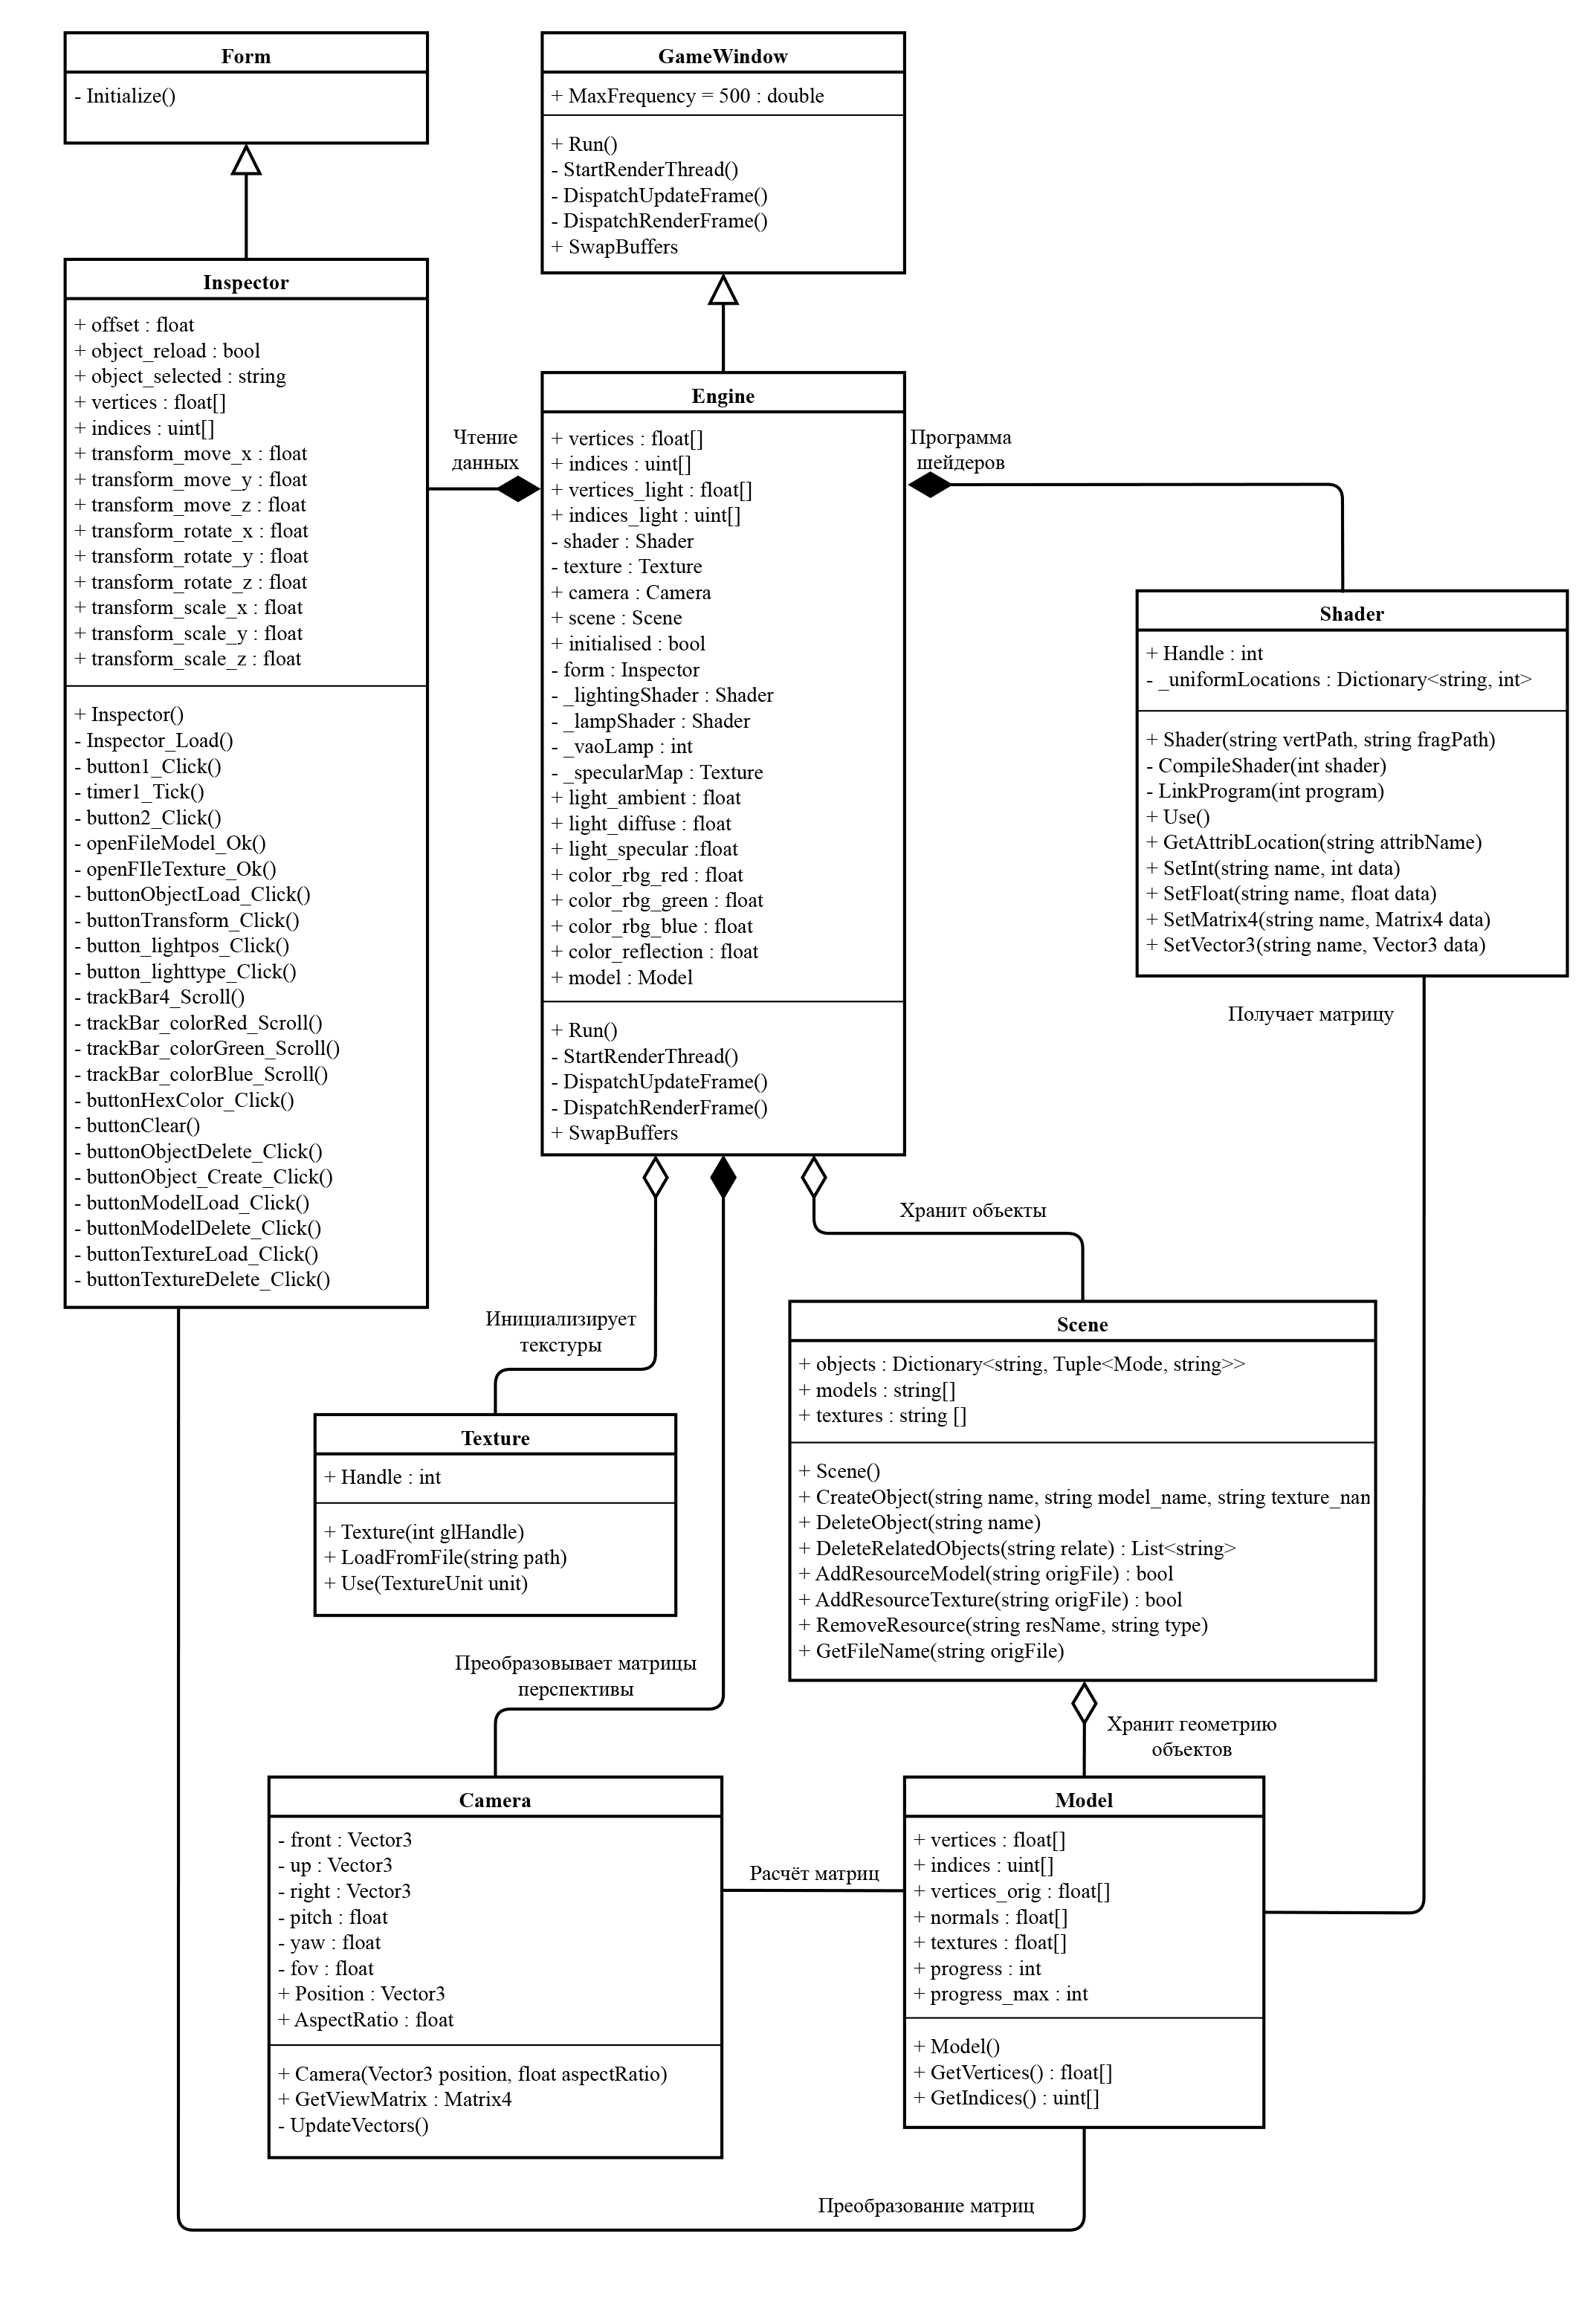
\includegraphics[width=1\linewidth]{diagram12.png}}
\caption{Диаграмма классов программы}
\label{diagram3:image}
\end{figure}

Все элементы программы имеют общий родительский элемент в виде главного класса - обработчика событий, который является главным элементом и центром всей программы.

\paragraph{Класс Model}

Является каркасом трёхмерной модели. Выполняет роль приёма, хранения и передачи массива трёхмерных данных для обработчика триангулярных примитивов. При создании выполняет чтение и преобразование в массивы вершин и индексов, загруженного файла с данными трёхмерного объекта.

\paragraph{Класс Texture}

При инициализации выделяет место в буффере памяти видеоадаптера для загруженной в программу текстуры, а также обрабатывает настройки параметров её отображения;

\paragraph{Класс Scene}

Выполняет роль хранилища моделей и изображений, а также выступает виртуальной сценой, на которой находятся все трёхмерные объекты и остальные элементы, учавствующие в визуализации. При инициализации выполняет загрузку данных массивов моделей и привязанных к ним файлов текстур, которые уже были раннее загружены в проект;

\paragraph{Класс Shader}

Программа настройки конечной визуализации, и при инициализации создаёт подпрограмму в общей графике, для преобразования растеризированного изображения внутри буффера памяти видеоадаптера, для отображения текстур и освещения;

\paragraph{Класс Camera}

Является матрицей преобразования, для корректного отображения перспективы виртуального трёхмерного вида сцены, и для того, чтобы конечный вид проекции сцены был перспективным, а не ортографическим;

\paragraph{Класс Model}

Представляет из себя основу проекта - графический движок, который инициализирует всю графику, принимает события ввода пользователя, отвечает за обновление кадров и управление всеми настройками, а также связывает все классы между собой;

\paragraph{Класс Inspector}

Часть пользовательского интерфейса, представляющего из себя окно взаимодействия между пользователем и программой. Служит для того, чтобы пользователь осуществлял загрузку собственных массивов трёхмерных данных моделей и текстур в проект, а также осуществлял указанные аффинные преобразования над загруженными моделями.

\paragraph{Класс GameWindow}

Также отдельно стоит указать класс GameWindow - это родительский класс для класса Engine. По своей сути он является измененным элементом класса Form от WindowsForms и не принимает прямого участия в работе проекта, но содержит формальные данные, необходимые для корректной инициализации главного окна проекта.

\subsubsection{Диаграмма компонентов}

Диаграмма компонентов - это структурная диаграмма языка унифицированного моделирования, она описывает особенности физического представления системы. Диаграмма компонентов позволяет определить архитектуру разрабатываемой системы, установив зависимости между программными компонентами.

Диаграмма компонентов предоставляет общую картину архитектуры системы, помогает разработчикам и архитекторам лучше понять ее структуру и взаимосвязи, а также является полезным инструментом для коммуникации и документирования архитектурных решений.

Диаграмма компонентов разрабатывается для следующих целей:
\begin{itemize}
	\item визуализация общей структуры исходного кода программной системы;
	\item спецификация исполнимого варианта программной системы;
	\item обеспечение многократного использования отдельных фрагментов программного кода;
	\item представление концептуальной и физической схем баз данных.
\end{itemize}

На рисунке \ref{diagram5:image} изображена диаграмма компонентов программной системы.
\begin{figure}[ht]
\center{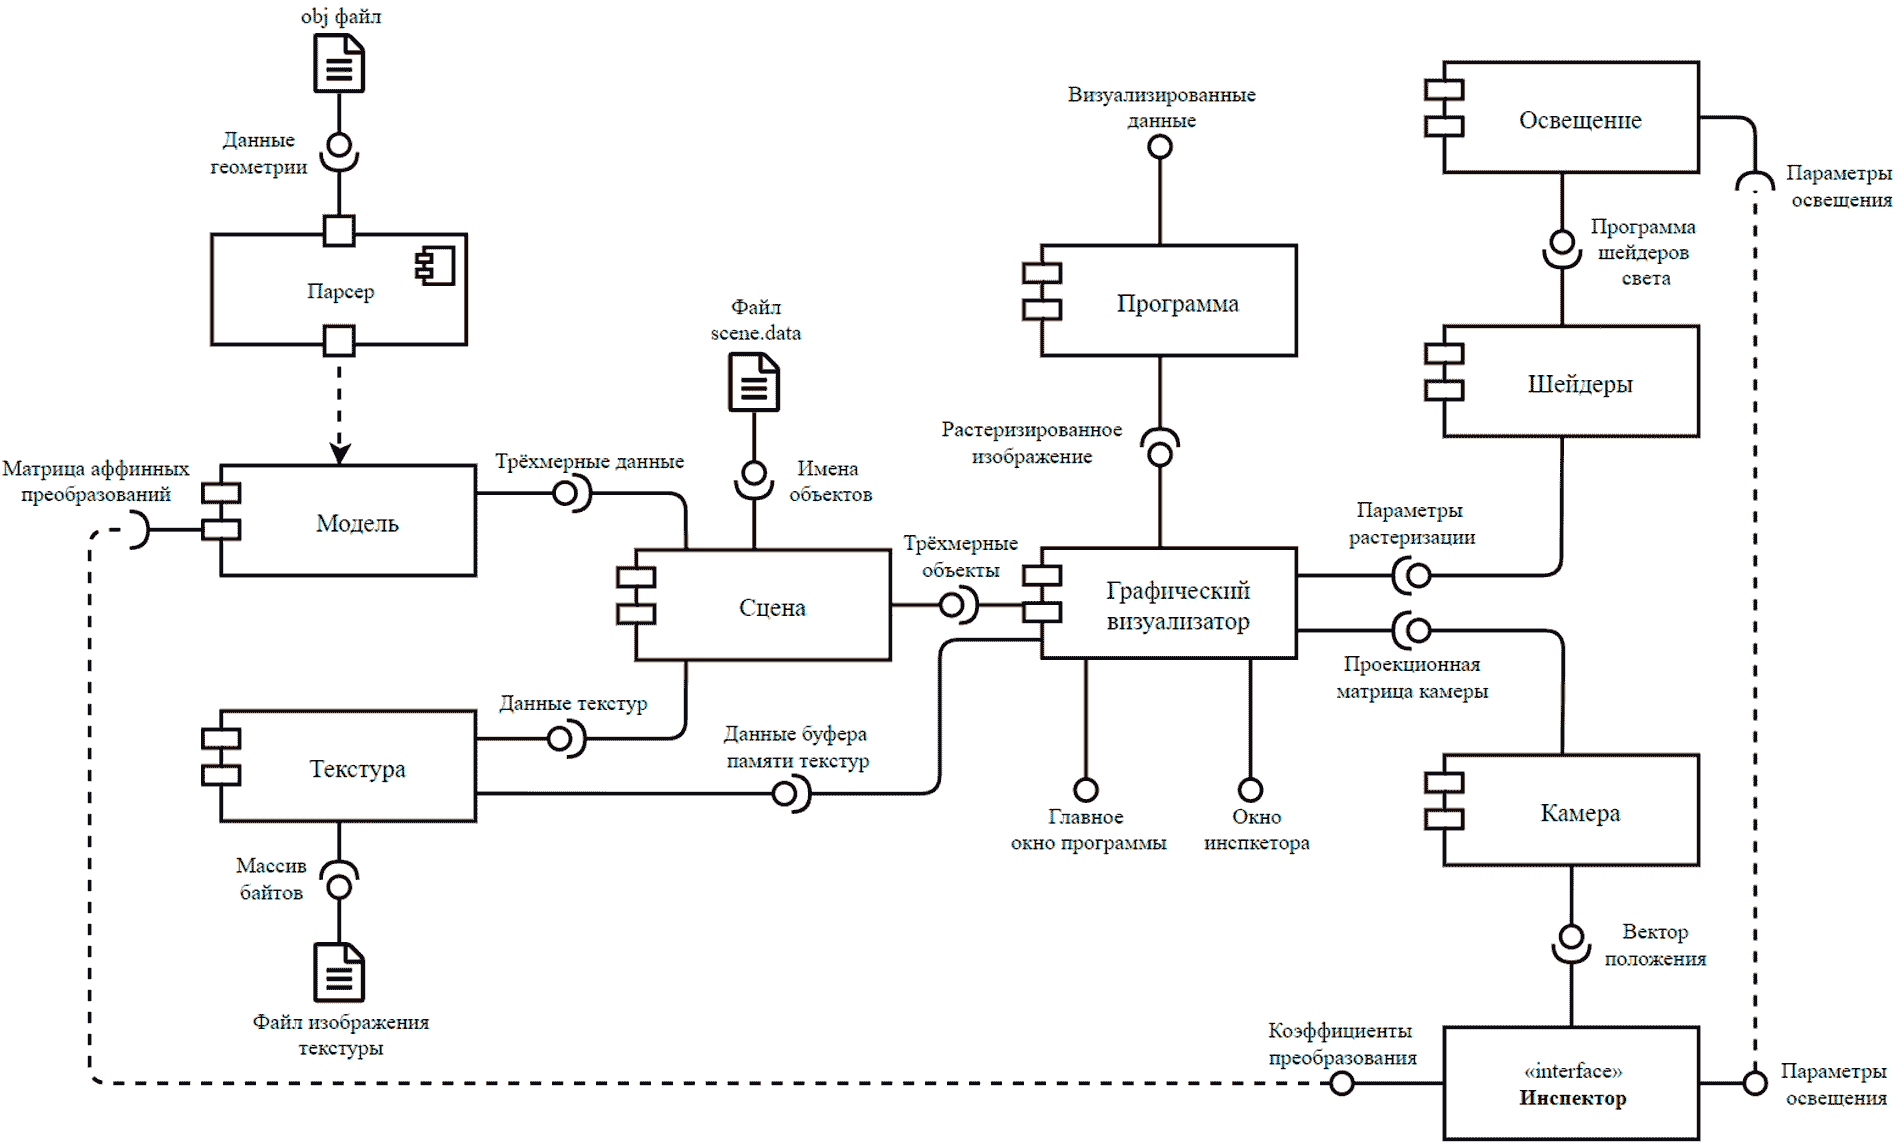
\includegraphics[width=1.025\linewidth]{diagram5.png}}
\caption{Диаграмма компонентов программы}
\label{diagram5:image}
\end{figure}

Данная диаграмма определяет общую архитектуру приложения, все его компоненты, а также устанавливает зависимости между ними в программной системе. Далее мы подробно опишем работу каждого компонента по отдельности.

\paragraph{Компонент Файл OBJ}

Является файлом с данными, расширения *.obj, содержащим данные трёхмерной геометрии объекта.

Предоставляет общий набор данных геометрии трёхмерной модели.

\paragraph{Компонент Парсер}

Синтаксический анализатор, преобразующий общий набор данных геометрии в отдельные массивы, подходящие по стандарту программной системы для корректной визуализации объектов.

Принимает общие данные геометрии трёхмерных моделей.

Является компонентом, зависимым от модуля Модель.

\paragraph{Компонент Модель}

Выполняет функцию обработки и хранения массивов трёхмерных данных. Преобразовывает, хранит и передаёт данные файла геометрии трёхмерного объекта.

Предоставляет массивы трёхмерных данных, понятных в интерпретации для программной среды.

\paragraph{Компонент Файл изображения текстуры}

Является файлом растрового изображения в форматах *.png или *.jpg.

Предоставляет закодированное изображение текстуры в виде массива байтов.

\paragraph{Компонент Текстура}

Обработчик изображения, который генерирует текстуру в системе и задаёт параметры для отрисовки и фильтрации изображения. Выделяет место в буффере текстур, а также привязывает ей определенный идентификатор в памяти буфера видеоадаптера.

Принимает массив байтов изображения текстуры.

Предоставляет общие данные текстуры в системе - её идентификатор и адрес в буфере памяти.

\paragraph{Компонент Файл scene.data}

Файл в который программа записывает и хранит данные идентификаторов, имён и ссылок на модели и текстуры.

Передаёт набор синтаксически размеченных строк, определяющих имена моделей и текстур.

\paragraph{Компонент Сцена}

Виртуальная сцена, которая представляет из себя словарь моделей и текстур, связывающий их идентификаторы в общую структуру объекта.

Принимает трёхмерные данные моделей, системы данные и параметры текстур, а также имён - идентификаторов моделей и текстур.

Передаёт обработанные и структурированные данные трёхмерных объектов, готовых к визуализации.

\paragraph{Компонент Инспектор}

Часть графического интерфейса программы, через который пользователь может производить взаимодействия над параметрами виртуальной среды и трёхмерными объектами, загруженными на виртуальную сцену.

Принимает данные вектора положения камеры.

Предоставляет коэффициенты для осуществления трансформации матриц аффинных преобразований. Также предоставляет параметры настройки освещения.

\paragraph{Компонент Камера}

Описывает матрицу перспективы, по которой происходит создание перспективы виртуальной среды.

Предоставляет проекционную матрицу перспективы.

\paragraph{Компонент Освещение}

Программа шейдера, отвечающая за обработку отражения света, а также уровня яркости грани модели, в зависимости от положения источника света.

Принимает параметры для настроек аттрибутов освещения.

Предоставляет программу шейдеров света.

\paragraph{Компонент Шейдеров}

Общая программа шейдеров, отвечающая за обработку отображения цвета и текстур вершин и граней моделей.

Принимает программу шейдеров света.

Предоставляет параметры шейдинга для финальной растеризации визуализированной сцены.

\paragraph{Модуль Графический визуализатор}

Главный блок программы, представляющий собой графический визуализатор, связывающий все модули программной среды, обрабатывая все необходимые данные для создания композиции и визуализации сцены трёхмерной среды.

Принимает обработанные массивы данных трёхмерных объектов, данные буфера памяти текстур, параметры программ шейдеров, а также матрицу проекции камеры.

Предоставляет графический интерфейс в виде главного окна программы и окна инспектора. Также передаёт конечное растрированное изображение в главный класс программы.

\paragraph{Компонент Программа}

Является начальным родительским компонентом всей программной среды, который осуществляет запуск приложения с определенными параметрами. Осуществляет запуск графического визуализатора с заданными аттрибутами.

Принимает данные графического визуализатора в виде растеризированного кадра.

Визуализирует растеризированную композицию кадра виртуальной сцены у пользователя на экране в главном окне программы.

\subsection{Описание файлов трёхмерных данных формата OBJ}
Формат файлов OBJ, или же Wavefront .obj файл - это формат файлов описания геометрии, разработанный в 1992 году компанией компьютерной графики Wavefront Technologies. Он содержит только 3D геометрию, а именно: позицию каждой вершины, связь координат текстуры с вершиной, направления нормалей, а также параметры, которые создают триангулярные примитивы. На основе файлов данного формата, завязан главный принцип работы разрабатываемой программной среды. 

Данный формат файла имеет следующие особенности:
\begin{itemize}
	\item он позволяет пользователям использовать файловое представление объектов сложной или неевклидовой формы, разделяя поверхность на треугольные грани, которые называются триангулярными примитивами. Данный процесс трасселяции упрощает процесс манипуляции, моделирования и визуализации, поскольку позволяет изменять каждую грань независимо от остальных;
	\item ещё одной важной особенностью является способность определять свойства поверхности трёхмерной геометрии объектов, такие как определение координат текстур и карты нормалей для шейдинга;
	\item OBJ поддерживает данные высокого разрешения, в сравнении со схожими форматами трёхмерных данных, к примеру, такими как STL;
	\item и в заключении, ещё одной особенностью данного формата является возможность хранения сразу нескольких текстур и цветов в одном объекте, в отличие от файлов, как в том же формате STL.
\end{itemize}

Несмотря на то, что данный формат расширения файлов используется уже более тридцати лет, он не является устаревшим, а даже более того - почти основным и универсальным форматом хранения данных трёхмерной геометрии. 

Существует множество способов открыть OBJ-файл и преобразовать его в различные другие форматы. Одним из вариантов является использование такого программного обеспечения, как 3DS Max, Solidworks, Cinema 4D или Blender, которое позволяет легко импортировать 3D-модели в формате OBJ, а затем преобразовывать и экспортировать их в любой необходимый формат.

Также данные объекта в OBJ-файле можно редактировать даже не запуская ни одно из программных обеспечений для трёхмерной графики, а просто открыв его в блокноте. Данный формат не закодирован какой-либо особой системой, и представлен в виде простого незашифрованного набора текста - данных трёхмерной геометрии. Пример содержания OBJ-файла представлен в ПРИЛОЖЕНИИ А.

\subsection{Описание работы парсера}

В результате необходимости импортирования и использования в программной среде файлов трёхмерных данных с расширением *.obj из внешней файловой системы устройства, возникла необходимость автоматизировать загрузку и интерпретацию этих данных для программы. Для решения данной задачи был разработан специальный алгоритм программы парсера.

Парсер, или же синтаксический анализатор - часть программы, которая преобразовывает текстовые входные данные в структурированный формат.

Исходя из этого, необходимо, чтобы парсер мог разделить все эти данные на отдельные массивы, которые будет использовать программа. В заключение вышесказанного, можно построить схему, по которой должен будет работать парсер, как показано на рис.~\ref{diagram4:image}, где изображена схема работы подпрограммы парсера.

\begin{figure}[ht]
	\center{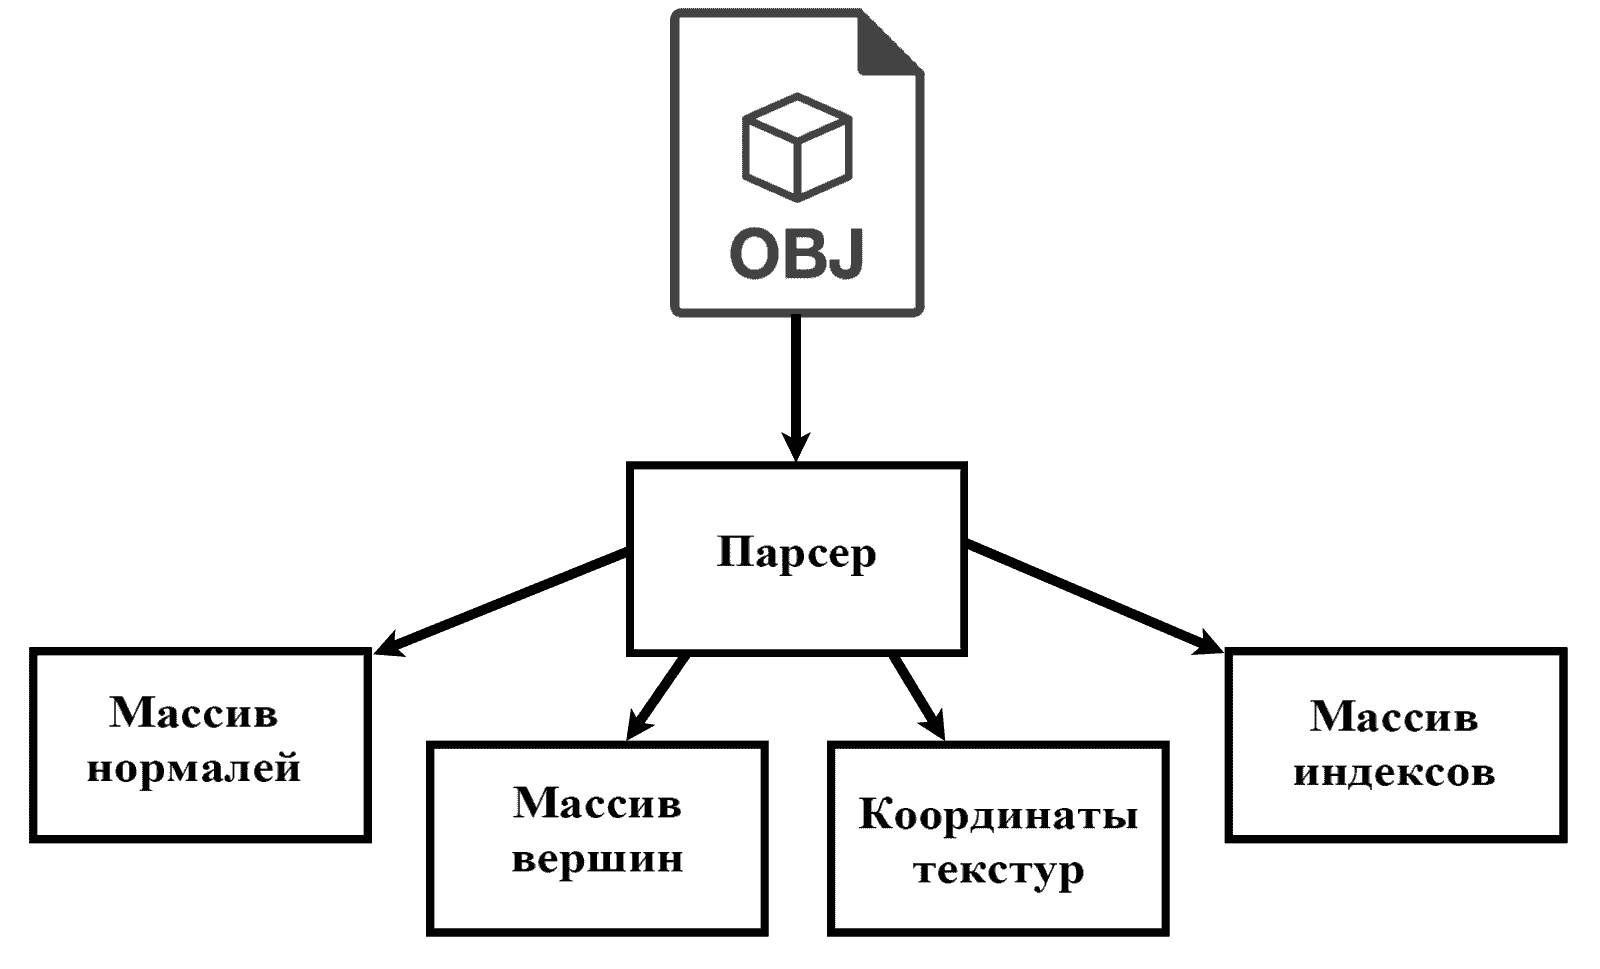
\includegraphics[width=1\linewidth]{diagram4.png}}
	\caption{Схема работы программы парсера}
	\label{diagram4:image}
\end{figure}

На данной схеме показано, на какие массивы данных разбивается OBJ-файл в результате синтаксического анализа парсера. Данные массивы необходимо будет использовать по отдельности, чтобы каждый был задействован в соответствующих модулях и подпрограммах программной среды.

Парсер не представляет собой отдельный независимый класс. Он является компонентом модуля, и его подпрограмма находится в классе Model. Это создаёт удобство в использовании данного класса, так как в следствии, каждый его элемент будет иметь возможность автоматически интерпретировать и структурировать данные геометрии своей модели в массивы трёхмерных данных, в результате чего, они сразу смогут структурироваться под стандарты программы, при инициализации элемента класса Model.

Фрагмент листинга кода парсера представлен в ПРИЛОЖЕНИИ Г.

\subsection{Система хранения данных внутри проекта}

Программная система имеет начальный набор данных - текстуры и файлы геометрии, чтобы пользователь мог начать ознакомление с программой со встроенных данных, без необходимости подгружать дополнительные файлы из системы для полноценной работы программы. В ситуации, в которой количество хранимых файлов приложением больше одного, возникла необходимость спроектировать структурированную систему индексирования и хранения всех данных, чтобы программа понимала, какие данные в текущий момент пользователь планирует использовать.
Для того, чтобы приложение могло работать с большим количеством данных и файлов, была разработана система хранения данных, которая имеет свои принципы и особенности. К файлам проекта программная система обращается через два файла данных - "<Objects.data"> и "<Resources.data">.

\subsubsection{Файл Resource.data}

В файле "<Resources.data"> программа записывает и считывает массив всех хранимых программой ресурсов - файлов геометрии и текстур. Каждая строка представляет собой отдельный ресурс - либо файл геометрии, либо текстуры, в которой записано их имя - относительный путь к файлам внутри проекта. Хранение ресурсов осуществляется по принципу листа, который проще говоря, является динамически расширяемым массивом данных, который можно расширять с конца. Данные ресурсы используются для дальнейшего представления объектов. Пример содержания и синтаксиса файла приведён в ПРИЛОЖЕНИИ В.

\subsubsection{Файл Objects.data}

В файле "<Objects.data"> программа записывает и считывает структуру объекта. Каждая строка файла представляет собой отдельный объект, который состоит из трёх частей - имени объекта, файла геометрии OBJ и файла изображения текстуры. Хранение объектов осуществляется по принципу словаря, где к каждому имени объекта привязаны свои определенные модели и текстуры, что собственно и является самими представлением объекта. Пример содержания и синтаксиса файла приведён в ПРИЛОЖЕНИИ В.

\subsection{Проектирование пользовательского интерфейса}

Графический прототип интерфейса, показанный на рис.~\ref{maket2:image} демонстрирует, какие элементы пользовательского интерфейса будут включены в конечную реализацию программы.

\begin{figure}[H]
\center{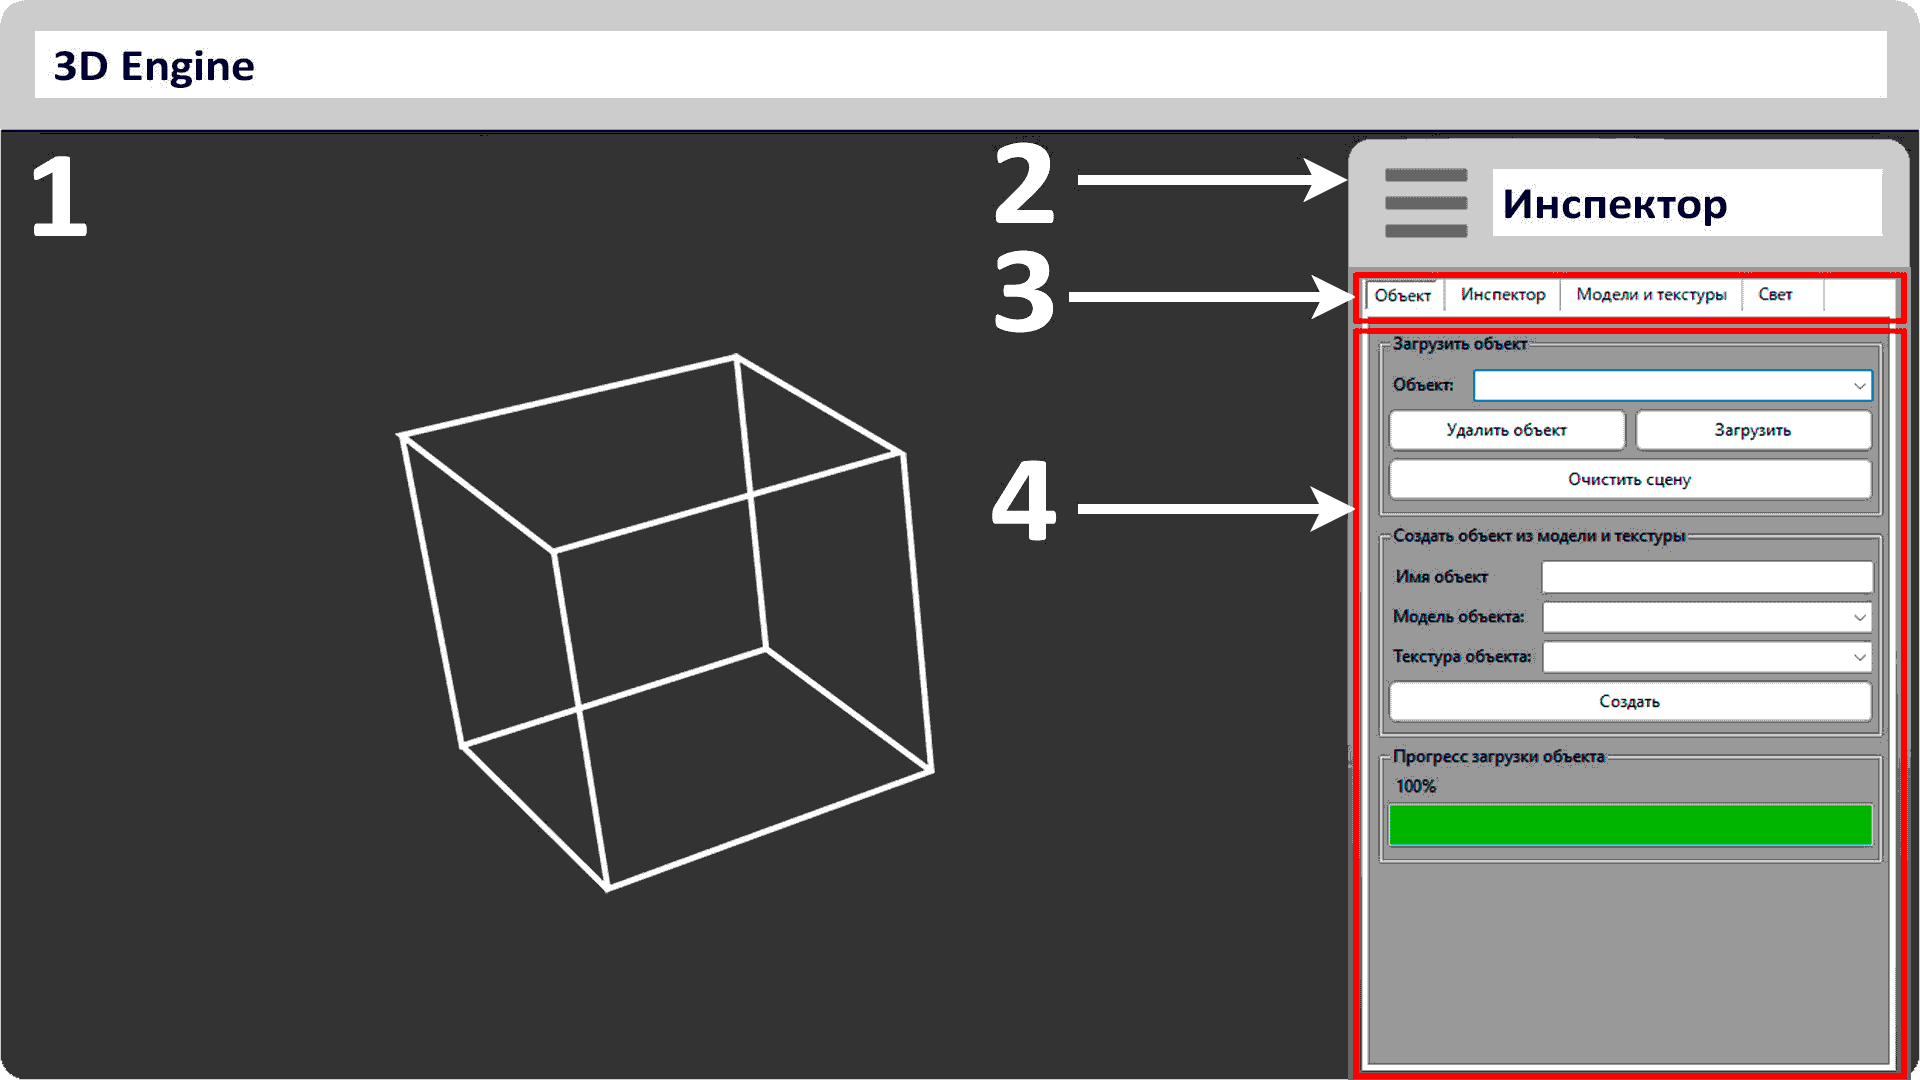
\includegraphics[width=1\linewidth]{maket2.png}}
\caption{Прототип пользовательского интерфейса}
\label{maket2:image}
\end{figure}

Описание элементов интерфейса, показанного на рис.~\ref{maket2:image}:
\begin{enumerate}
	\item Главное окно программы. Выводит визуализированные данные на экран.
	\item Окно инспектора.
	\item Вкладки окон инспектора.
	\item Активное меню вкладки инспектора.
\end{enumerate}

\subsubsection{Главное окно программы}

Главное окно программы представляет из себя виртуальную трёхмерную среду с одноцветным фоном. Оно служит для отображения визуализации трёхмерных моделей, которые пользователь загрузит в программу. Также данное окно является частью пользовательского интерфейса с интуитивной функцией ввода - пользователь может управлять направлением перспективы взгляда камеры, зажав правую кнопку мыши и направляя курсор в нужную сторону, чтобы управлять камерой и осматриваться в виртуальном пространстве. А используя колесо прокрутки, пользователь может отдалять и приближать угол обзора.

Управление перемещением камеры в пространстве также осуществляется в главном окне программы, с помощью клавиатуры:
\begin{itemize}
	\item клавиша «W» – переместить камеру вперёд по направлению взгляда;
	\item клавиша «A» – переместить камеру вправо относительно направления взгляда;
	\item клавиша «S» – переместить камеру назад по направлению взгляда;
	\item клавиша «D» – переместить камеру влево относительно направления взгляда;
	\item клавиша «левый Shift» – поднять камеру вверх, по координате +Y;
	\item клавиша «левый Ctrl» – опустить камеру вниз, по координате -Y;
\end{itemize}

\subsubsection{Окно инспектора}

Инспектор - это дополнительное окно, расположенное по краю справа, поверх главного окна. Оно служит вспомогательным элементом интерфейса, чтобы пользователь мог взаимодействовать и управлять элементами внутри виртуальной сцены. Например, выполнять преобразование массива данных трёхмерной модели - перемещать её в пространстве, наклонять под определённым углом и прозводить растяжение или сжатие, и всё это по всем трём координатам.

\subsubsection{Вкладки окон инспектора}

Меню со вкладками окон инспектора, где пользователь может выбрать одну трёх вкладок, чтобы переключать и менять содержание активного меню инспектора.

\subsubsection{Активное меню вкладки инспектора}

Показывает основной интерфейс меню инспектора. Инспектор имеет три разных активных меню, и содержание окна инспектора будет меняться, в зависимости от выбранной вкладки.

\paragraph{Вкладка "<Объект">}
Вкладка "<Объект"> - в данной вкладке пользователь может выбрать из выпадающего списка объект, который он хочет загрузить и визуализировать на виртуальной сцене. Также данная вкладка имеет ещё один важный раздел, в котором пользователь может создать новый объект внутри проекта - связав выбранный файл из списка моделей и файл из списка текстур, имеющихся внутри проекта, в новую сущность, дав имя получившемуся объекту.

\paragraph{Вкладка "<Инспектор">}
Вкладка "<Инспектор"> - это информационная вкладка, в которой показаны точные координаты и наклон камеры, а также в которой пользователь может осуществить аффиинные преобразования над загруженной моделью на сцену в данный момент и узнать данные об уже раннее произведенных преобразованиях над моделью: смещении, наклона и масштабировании.

\paragraph{Вкладка "<Модели и текстуры">}
Вкладка "<Модели и текстуры"> содержит весь список доступных моделей и текстур в программе, загруженных пользователем. Также в ней пользователь может осуществлять непосредственно саму загрузку массивов трёхмерных данных с расширением *.obj в программу и изображений текстур с расширением *.png и *.jpg. Также в данной вкладке пользователь может удалить уже существующие файлы моделей и текстур из проекта.

\paragraph{Вкладка "<Свет">}
Во вкладке "<Свет"> пользователю представлены текущие настройки параметров всех типов освещений, излучаемых источником света, которые пользователь может свободно изменять, чтобы получить желаемый результат отрисовки освещения отраженного и рассеянного света то поверхности объекта.